% Baccalauréat malgache, série C, 2013 : corrigé.
\TCDBacAttribution{C}{2013}
\providecommand{\cm}{~\mathrm{cm}}
\providecommand{\Plan}{(\mathscr{P})}
\providecommand{\dx}{~\mathrm{d}x}
\providecommand{\dt}{\mathrm{d}t}
\providecommand{\Ouv}{(O;\vec{u},\vec{v})}
\providecommand{\mes}[2]{\mathrm{mes}\left( \widehat{ \overrightarrow{#1} ; \overrightarrow{#2} } \right)}
\providecommand{\D}{(\mathscr{D})}
\providecommand{\Courbe}{(\mathscr{C})}
\providecommand{\bary}[1]{\mathrm{bar}\left\lbrace #1 \right\rbrace}
\providecommand{\Angl}[2]{\left( \widehat{ \overrightarrow{#1} , \overrightarrow{#2} } \right)}
%
%%%%%%%%%%%%%%%%%%%%%%%%%%%%%%%%%%%%%%%%%%%%%%%%%%%%%%%%%%%%%%%%%%%%%%%%%%%%%%%%%%%%%%%%%%%%%%%%%%%%%%%%%%%%%%%%%%%%%%%%%%%%%%%%
\noindent \underline{\textsc{\textbf{Exercice}}} (4 points)
\begin{description}
	\item[A.] \underline{Arithmétique}
	\begin{enumerate}
		\item \vln{Valeur de $n$ :}
			En base $4$ : $A = 1 \times 16 + 2 \times 4 + 1 = 25$. En base $n$ : $A = 2n^2 + 2n + 1$ (avec $n \geq 3$ car le chiffre $2$ apparaît).
			$2n^2 + 2n + 1 = 25 \iff n^2 + n - 12 = 0 \iff (n - 3)(n + 4) = 0$.
			\par\noindent\ansbox{$n = 3$ (vérification : $2 \times 9 + 2 \times 3 + 1 = 25$).}
		\item \vln{Divisibilité par $11$ :}
			\textit{Telle qu'elle est écrite, la propriété est fausse : pour $n = 1$, $2^6 + 9^2 = 64 + 81 = 145 = 11 \times 13 + 2$.
			L'énoncé voulu est très probablement $2^{6n+1} + 9^{n+1} \equiv 0 \ [11]$ (même exercice qu'en 2008), que l'on démontre.}

			$2^6 = 64 = 5 \times 11 + 9 \equiv 9 \pmod{11}$, donc $2^{6n+1} = 2 \times \left(2^6\right)^n \equiv 2 \times 9^n$.
			Ainsi $2^{6n+1} + 9^{n+1} \equiv 2 \times 9^n + 9 \times 9^n = 11 \times 9^n \equiv 0 \pmod{11}$.
			\par\noindent\ansbox{Pour tout $n \in \mathbb{N}$, $2^{6n+1} + 9^{n+1} \equiv 0 \ [11]$.}
		\item \vln{Système $\pgcd{a}{b} = 6$, $PPCM(a;b) = 240$ :}
			On écrit $a = 6a'$, $b = 6b'$ avec $\pgcd{a'}{b'} = 1$ ; alors $PPCM(a;b) = 6a'b'$, d'où $a'b' = 40 = 2^3 \times 5$.
			Les couples d'entiers premiers entre eux de produit $40$ sont $(1,40)$, $(8,5)$, $(5,8)$, $(40,1)$
			($(2,20)$ et $(4,10)$ sont exclus : ils ne sont pas premiers entre eux).
			\par\noindent\ansbox{$(a,b) \in \{(6,240) \, ; (48,30) \, ; (30,48) \, ; (240,6)\}$.}
	\end{enumerate}
	\item[B.] \underline{Probabilité}
	On suppose que chaque boule est placée au hasard dans l'une des $n$ boîtes, indépendamment des autres : un placement est une application de l'ensemble des boules dans l'ensemble des boîtes, et les $n^n$ placements sont équiprobables.
	\begin{enumerate}
		\item Pour $n = 4$ : $4^4 = 256$ placements.
		\begin{description}
			\item[E :] \vln{Une boule par boîte :}
				Les placements sont alors des bijections : $4! = 24$. $P(E) = \frac{24}{256}$, soit \par\noindent\ansbox{$P(E) = \frac{3}{32}$.}
			\item[F :] \vln{Chaque boule dans la boîte de même numéro :}
				un seul placement : \par\noindent\ansbox{$P(F) = \frac{1}{256}$.}
			\item[G :] \vln{Exactement deux boules dans la boîte 1 :}
				on choisit ces deux boules ($\Comb{4}{2} = 6$ choix), les deux autres vont dans les boîtes 2, 3 ou 4 ($3^2 = 9$ choix) :
				$P(G) = \frac{54}{256}$, soit \par\noindent\ansbox{$P(G) = \frac{27}{128}$.}
		\end{description}
		\item
		\begin{enumerate}
			\item \vln{Expression de $P_n(k)$ :}
				Choisir les $k$ boules de la boîte 1 : $\Comb{n}{k}$ façons ; placer chacune des $n - k$ autres dans l'une des $n - 1$ autres boîtes : $(n-1)^{n-k}$ façons.
				\[
					P_n(k) = \frac{\Comb{n}{k}(n-1)^{n-k}}{n^n} = \Comb{n}{k}\left(\frac{1}{n}\right)^k \left(\frac{n-1}{n}\right)^{n-k} .
				\]
				\par\noindent\ansbox{$P_n(k) = \Comb{n}{k}\left(\frac{1}{n}\right)^k\left(1 - \frac{1}{n}\right)^{n-k}$}
				(loi binomiale : chaque boule tombe dans la boîte 1 avec la probabilité $\frac{1}{n}$).
			\item \vln{Identité :}
				Les événements « la boîte 1 contient $k$ boules », $k = 0, \ldots, n$, forment une partition, donc $\sum_{k=0}^{n} P_n(k) = 1$, soit
				$\sum_{k=0}^{n} \frac{\Comb{n}{k}(n-1)^{n-k}}{n^n} = 1$.
				\par\noindent\ansbox{$\sum_{k=0}^{n} \Comb{n}{k}(n-1)^{n-k} = n^n$}
				(c'est aussi la formule du binôme : $(1 + (n-1))^n$).
		\end{enumerate}
	\end{enumerate}
\end{description}
%%%%%%%%%%%%%%%%%%%%%%%%%%%%%%%%%%%%%%%%%%%%%%%%%%%%%%%%%%%%%%%%%%%%%%%%%%%%%%%%%%%%%%%%%%%%%%%%%%%%%%%%%%%%%%%%%%%%%%%%%%%%%%%%
\noindent \underline{\textsc{\textbf{PROBLEME I}}} (7 points)
\begin{description}
	\item[Partie A]
	\begin{enumerate}
		\item \vln{Nature de $r_B \circ r_A$ :}
			On note $\Delta_1$ la droite passant par $A$ telle que $\left(\Delta_1 , (AB)\right) = \frac{\pi}{4}$ et $\Delta_2$ la droite passant par $B$ telle que $\left((AB) , \Delta_2\right) = \frac{\pi}{4}$
			(angles de droites). Alors $r_A = s_{(AB)} \circ s_{\Delta_1}$ et $r_B = s_{\Delta_2} \circ s_{(AB)}$, donc
			$r_B \circ r_A = s_{\Delta_2} \circ s_{\Delta_1}$.
			$\Delta_2$ est parallèle à $(AC)$ et $\Delta_1$ à $(BD)$ ; elles sont perpendiculaires et se coupent en un point $K$ ;
			$s_{\Delta_2} \circ s_{\Delta_1}$ est la rotation de centre $K$ et d'angle $2 \times \frac{\pi}{2} = \pi$.
			Le triangle $AKB$ est rectangle isocèle en $K$, situé de l'autre côté de $(AB)$ par rapport à $I$ : $K$ est le symétrique de $I$ par rapport à $(AB)$.
			\par\noindent\ansbox{$r_B \circ r_A$ est la symétrie centrale de centre $K$, symétrique de $I$ par rapport à $(AB)$.}
			(Contrôle avec le repère de la question 2 : $r_B \circ r_A (z) = i(iz - 1) + 1 = -z + 1 - i$, de point fixe $\frac{1 - i}{2}$.)
		\item Dans le repère $(A;\vec{u},\vec{v})$ : $z_A = 0$, $z_B = 1$, $z_C = 1 + i$, $z_D = i$.
		\begin{enumerate}
			\item \vln{Forme algébrique de $a$ :}
				$a = \frac{0 - (1+i)}{1 - (1+i)} = \frac{-1 - i}{-i} = \frac{1 + i}{i} = -i(1 + i)$, soit \par\noindent\ansbox{$a = 1 - i$.}
			\item \vln{Similitude de centre $C$ transformant $B$ en $A$ :}
				Elle s'écrit $z' - z_C = a(z - z_C)$ puisque $z_A - z_C = a(z_B - z_C)$.
				$a = 1 - i = \sqrt{2}\,\expo{-i\frac{\pi}{4}}$ : \par\noindent\ansbox{rapport $\sqrt{2}$, angle $-\frac{\pi}{4}$.}
		\end{enumerate}
		\item
		\begin{enumerate}
			\item \vln{$f$ est un antidéplacement :}
				$t_{\overrightarrow{AC}}$ et $r_A$ sont des déplacements, $\mathscr{S}_{(AD)}$ est un antidéplacement ; la composée de deux déplacements et d'un antidéplacement est un antidéplacement.
				\par\noindent\ansbox{$f$ est un antidéplacement.}
			\item \vln{Nature de $f$ :}
				$\left((AC),(AD)\right) = \frac{\pi}{4}$, donc $r_A = \mathscr{S}_{(AD)} \circ \mathscr{S}_{(AC)}$. Alors
				$f = \mathscr{S}_{(AD)} \circ \mathscr{S}_{(AD)} \circ \mathscr{S}_{(AC)} \circ t_{\overrightarrow{AC}} = \mathscr{S}_{(AC)} \circ t_{\overrightarrow{AC}}$.
				Le vecteur $\overrightarrow{AC}$ dirige l'axe $(AC)$ :
				\par\noindent\ansbox{$f$ est la symétrie glissée d'axe $(AC)$ et de vecteur $\overrightarrow{AC}$.}
			\item \vln{Expression complexe :}
				La réflexion d'axe $(AC)$ (droite $y = x$) s'écrit $z \mapsto i\bar{z}$ ; la translation, $z \mapsto z + 1 + i$. Donc
				$f(z) = i\,\overline{(z + 1 + i)} = i\bar{z} + i(1 - i)$.
				\par\noindent\ansbox{$f : z' = i\bar{z} + 1 + i$.}
				(Vérification directe : $t : z + 1 + i$, $r_A : iz + i - 1$, $\mathscr{S}_{(AD)} : z \mapsto -\bar{z}$, d'où $f(z) = -\overline{(iz + i - 1)} = i\bar{z} + i + 1$.)
		\end{enumerate}
	\end{enumerate}
	\item[Partie B]
	\begin{enumerate}
		\item \vln{Résolution de $(E_\theta)$ et $(E'_\theta)$ :}
			Discriminant réduit : $\Delta' = \cos^2\theta - 1 = -\sin^2\theta = (i\sin\theta)^2$. Les solutions sont $t = \cos\theta \pm i\sin\theta$ :
			\par\noindent\ansbox{$(E_\theta)$ : $t_1 = \expo{i\theta}$, $t_2 = \expo{-i\theta}$.}
			$(E'_\theta)$ équivaut à $z^2 = \expo{i\theta}$ ou $z^2 = \expo{-i\theta}$ (on pose $t = z^2$) :
			\par\noindent\ansbox{$(E'_\theta)$ : $z \in \left\{\expo{i\frac{\theta}{2}} \, ; -\expo{i\frac{\theta}{2}} \, ; \expo{-i\frac{\theta}{2}} \, ; -\expo{-i\frac{\theta}{2}}\right\}$.}
		\item Pour $\theta = \frac{\pi}{3}$, les solutions sont $\pm\expo{i\frac{\pi}{6}}$ et $\pm\expo{-i\frac{\pi}{6}}$, soit $\pm\frac{\sqrt{3}}{2} \pm \frac{1}{2}i$.
			$\Re{z_A} < 0$ et $\Im{z_B} = -\Im{z_A} < 0$ donnent $\Im{z_A} > 0$ :
			\par\noindent\ansbox{$z_A = -\frac{\sqrt{3}}{2} + \frac{1}{2}i$, $z_B = \frac{\sqrt{3}}{2} - \frac{1}{2}i$, $z_C = \frac{\sqrt{3}}{2} + \frac{1}{2}i$, $z_D = -\frac{\sqrt{3}}{2} - \frac{1}{2}i$.}
		\begin{enumerate}
			\item \vln{Figure (cercle de rayon $3\cm$) :}
				Les quatre points sont sur le cercle unité ; $A$ et $B$ sont diamétralement opposés, ainsi que $C$ et $D$.
				\textit{Le quadrilatère convexe est donc $ACBD$ (rectangle de diagonales $[AB]$ et $[CD]$) ; c'est lui que l'énoncé appelle « rectangle $ABCD$ ».}
				\begin{center}
				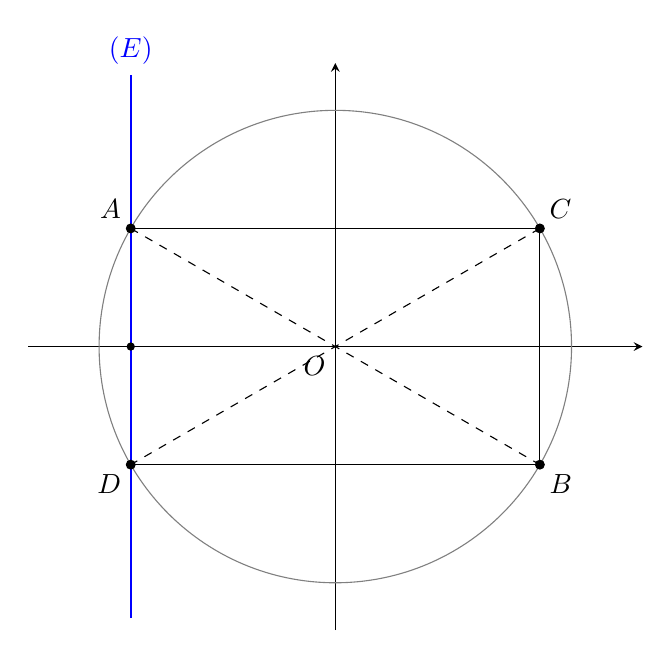
\begin{tikzpicture}[scale=3,>=stealth]
					\draw[->] (-1.3,0) -- (1.3,0); \draw[->] (0,-1.2) -- (0,1.2);
					\draw[gray] (0,0) circle (1);
					\coordinate (A) at (-0.866,0.5); \coordinate (B) at (0.866,-0.5); \coordinate (C) at (0.866,0.5); \coordinate (D) at (-0.866,-0.5);
					\draw (A) -- (C) -- (B) -- (D) -- cycle;
					\draw[dashed] (A) -- (B) (C) -- (D);
					\draw[blue,thick] (-0.866,-1.15) -- (-0.866,1.15) node[above] {$(E)$};
					\fill (-0.866,0) circle (0.5pt);
					\foreach \P/\pos in {A/above left,B/below right,C/above right,D/below left}
						\fill (\P) circle (0.6pt) node[\pos] {$\P$};
					\node[below left] at (0,0) {$O$};
				\end{tikzpicture}
				\end{center}
			\item \vln{Cas du carré :}
				Pour $\theta$ quelconque, les quatre points $\pm\expo{\pm i\frac{\theta}{2}}$ forment un rectangle inscrit dans le cercle unité (deux diamètres) ;
				c'est un carré si et seulement si ces diamètres sont perpendiculaires, c'est-à-dire si l'angle entre $\expo{-i\frac{\theta}{2}}$ et $\expo{i\frac{\theta}{2}}$, égal à $\theta$, vaut $\frac{\pi}{2}$ modulo $\pi$.
				\par\noindent\ansbox{Carré pour $\theta = \frac{\pi}{2}$ (plus généralement $\theta \equiv \frac{\pi}{2} \pmod{\pi}$).}
		\end{enumerate}
		\item
		\begin{enumerate}
			\item \vln{$\overrightarrow{AG_\lambda}$ :}
				La somme des poids vaut $\lambda^2 + 1 + \lambda - \lambda = \lambda^2 + 1 > 0$ : $G_\lambda$ existe, et
				$\overrightarrow{AG_\lambda} = \frac{\lambda\overrightarrow{AB} - \lambda\overrightarrow{AD}}{\lambda^2 + 1} = \frac{\lambda}{\lambda^2 + 1}\overrightarrow{DB}$.
				\par\noindent\ansbox{$\overrightarrow{AG_\lambda} = -\frac{\lambda}{\lambda^2 + 1}\,\overrightarrow{BD}$.}
			\item \vln{Ensemble $(E)$ :}
				Pour $\lambda = 1$, $S_1 = \{(A,2);(B,1);(D,-1)\}$ et $2\overrightarrow{MA} + \overrightarrow{MB} - \overrightarrow{MD} = 2\overrightarrow{MG_1}$ ;
				pour $\lambda = -1$, $S_{-1} = \{(A,2);(B,-1);(D,1)\}$ et $2\overrightarrow{MA} - \overrightarrow{MB} + \overrightarrow{MD} = 2\overrightarrow{MG_{-1}}$.
				La condition s'écrit $MG_1 = MG_{-1}$ : $(E)$ est la médiatrice de $[G_1G_{-1}]$.
				Or $\overrightarrow{AG_1} = -\frac{1}{2}\overrightarrow{BD}$ et $\overrightarrow{AG_{-1}} = \frac{1}{2}\overrightarrow{BD}$ : $A$ est le milieu de $[G_1G_{-1}]$ et $(G_1G_{-1}) \parallel (BD)$.
				\par\noindent\ansbox{$(E)$ est la droite passant par $A$ et perpendiculaire à $(BD)$.}
				Ici $z_D - z_B = -\sqrt{3}$ : $(BD)$ est horizontale, donc $(E)$ est la droite verticale $x = -\frac{\sqrt{3}}{2}$, c'est-à-dire la droite $(AD)$ (tracée sur la figure).
		\end{enumerate}
	\end{enumerate}
\end{description}
%%%%%%%%%%%%%%%%%%%%%%%%%%%%%%%%%%%%%%%%%%%%%%%%%%%%%%%%%%%%%%%%%%%%%%%%%%%%%%%%%%%%%%%%%%%%%%%%%%%%%%%%%%%%%%%%%%%%%%%%%%%%%%%%
\noindent \underline{\textsc{\textbf{PROBLEME II}}} (9 points)
\begin{description}
	\item[Partie A]
	\begin{enumerate}
		\item
		\begin{enumerate}
			\item \vln{Continuité en $1$ :}
				$f(1) = (3 - 3)\expo{-1} = 0$ ; $\lim_{x\to 1^-} \left(x^2 - 1 - 2\ln x\right) = 1 - 1 - 0 = 0$ ; à droite, $f$ est continue (produit de fonctions continues).
				\par\noindent\ansbox{$f$ est continue en $1$.}
			\item \vln{Dérivabilité en $1$ :}
				À gauche, $x \mapsto x^2 - 1 - 2\ln x$ est dérivable en $1$ de dérivée $2x - \frac{2}{x}$, qui vaut $0$ en $1$ : $f'_g(1) = 0$.
				À droite, $x \mapsto (3x - 3)\expo{-x}$ a pour dérivée $3\expo{-x} - (3x - 3)\expo{-x} = (6 - 3x)\expo{-x}$, qui vaut $\frac{3}{e}$ en $1$ : $f'_d(1) = \frac{3}{e}$.
				\par\noindent\ansbox{$f$ n'est pas dérivable en $1$ ($f'_g(1) = 0 \neq f'_d(1) = \frac{3}{e}$) : point anguleux.}
				Demi-tangentes : horizontale à gauche ; de coefficient directeur $\frac{3}{e}$ à droite.
		\end{enumerate}
		\item
		\begin{enumerate}
			\item \vln{Sens de variation :}
				Sur $]0;1[$ : $f'(x) = 2x - \frac{2}{x} = \frac{2(x^2 - 1)}{x} < 0$ : $f$ est strictement décroissante.
				Sur $]1;+\infty[$ : $f'(x) = 3(2 - x)\expo{-x}$ : $f$ est strictement croissante sur $[1;2]$ et strictement décroissante sur $[2;+\infty[$.
			\item \vln{Tableau de variation :}
				$\lim_{x\to 0^+} f(x) = +\infty$ (car $-2\ln x \to +\infty$) ; $f(2) = 3\expo{-2} \approx 0{,}41$ ;
				$\lim_{x\to+\infty} (3x - 3)\expo{-x} = 3\frac{x}{\expo{x}} - \frac{3}{\expo{x}} \to 0$.
				\[
				\begin{array}{c|ccccccc}
					x & 0 & & 1 & & 2 & & +\infty \\ \hline
					f'(x) & & - & 0 \,\|\, \frac{3}{e} & + & 0 & - & \\ \hline
					 & +\infty & & & & 3\expo{-2} & & \\
					f & & \searrow & & \nearrow & & \searrow & \\
					 & & & 0 & & & & 0
				\end{array}
				\]
		\end{enumerate}
		\item
		\begin{enumerate}
			\item \vln{Point d'inflexion :}
				Sur $]0;1[$, $f''(x) = 2 + \frac{2}{x^2} > 0$ : $(C)$ est convexe, pas d'inflexion.
				Sur $]1;+\infty[$, $f''(x) = -3\expo{-x} - (6 - 3x)\expo{-x} = (3x - 9)\expo{-x}$, qui s'annule en $3$ en changeant de signe.
				En $1$, $f$ n'est pas dérivable, il n'y a pas de tangente : ce n'est pas un point d'inflexion.
				$f(3) = 6\expo{-3}$.
				\par\noindent\ansbox{Unique point d'inflexion : $I\left(3 \, ; 6\expo{-3}\right) \approx (3 \, ; 0{,}30)$.}
			\item \vln{Tangente $(T)$ en $I$ :}
				$f'(3) = -3\expo{-3}$, donc $y = -3\expo{-3}(x - 3) + 6\expo{-3}$.
				\par\noindent\ansbox{$(T) : y = 3\expo{-3}(5 - x)$ (avec $\expo{-3} = 0{,}05$ : $y = 0{,}15(5 - x)$).}
			\item \vln{Tracé (figure réduite : $2\cm$ pour une unité au lieu de $4\cm$) :}
				Valeurs : $f(0{,}2) \approx 2{,}26$ ; $f(0{,}5) \approx 0{,}64$ ; $f(2) \approx 0{,}41$ ; $f(3) \approx 0{,}30$ ; $f(5) \approx 0{,}08$.
				\begin{center}
				\begin{tikzpicture}[x=2cm,y=2cm,>=stealth]
					\draw[->] (-0.2,0) -- (6.2,0) node[below] {$x$};
					\draw[->] (0,-0.2) -- (0,3.1) node[left] {$y$};
					\foreach \t in {1,2,3,4,5,6} \draw (\t,0.03) -- (\t,-0.03) node[below] {\small $\t$};
					\foreach \t in {1,2,3} \draw (0.03,\t) -- (-0.03,\t) node[left] {\small $\t$};
					\node[below left] at (0,0) {$O$};
					\draw[blue,thick] plot[domain=0.14:1,samples=80] (\x,{\x*\x-1-2*ln(\x)});
					\draw[blue,thick] plot[domain=1:6,samples=100] (\x,{(3*\x-3)*exp(-\x)});
					\draw[red] (1.2,0.57) -- (5.8,-0.12) node[right] {$(T)$};
					\draw[gray] (0.6,0) -- (1,0);
					\draw[gray] (1,0) -- (1.35,0.386);
					\fill (3,0.2987) circle (1.2pt) node[above right] {$I$};
					\node[blue] at (0.55,1.6) {$(C)$};
				\end{tikzpicture}
				\end{center}
		\end{enumerate}
	\end{enumerate}
	\item[Partie B]
	Sur $]0;1]$, $f(t) = t^2 - 1 - 2\ln t$ (la formule donne aussi $f(1) = 0$).
	\begin{enumerate}
		\item
		\begin{enumerate}
			\item \vln{Calcul de $I(\lambda)$ :}
				Par parties avec $u(t) = \ln t$, $v'(t) = 1$ : $\int_\lambda^1 \ln t\,\dt = \left[t\ln t\right]_\lambda^1 - \int_\lambda^1 1\,\dt = -\lambda\ln\lambda - (1 - \lambda)$.
				Donc
				$I(\lambda) = \left[\frac{t^3}{3} - t\right]_\lambda^1 - 2\left(-\lambda\ln\lambda - 1 + \lambda\right) = -\frac{2}{3} - \frac{\lambda^3}{3} + \lambda + 2\lambda\ln\lambda + 2 - 2\lambda$.
				\par\noindent\ansbox{$I(\lambda) = \frac{4}{3} - \lambda - \frac{\lambda^3}{3} + 2\lambda\ln\lambda$.}
			\item \vln{Limite :}
				$\lim_{\lambda\to 0^+} \lambda\ln\lambda = 0$, donc \par\noindent\ansbox{$\lim_{\lambda\to 0} I(\lambda) = \frac{4}{3}$.}
		\end{enumerate}
		\item \textit{L'énoncé contient deux coquilles : en (b) l'intégrale est $\int_{\frac{1}{n}}^{1} f(t)\,\dt$ (et non $\int_{\frac{1}{n}}^{\frac{1}{n}}$), et en (c) il faut lire
			$I\left(\frac{1}{n}\right) + \frac{1}{n} f\left(\frac{1}{n}\right)$ à droite.}
		\begin{enumerate}
			\item \vln{Encadrement :}
				$f$ est décroissante sur $]0;1]$. Pour $t \in \left[\frac{k}{n} ; \frac{k+1}{n}\right]$ (avec $1 \leq k \leq n-1$) :
				$f\left(\frac{k+1}{n}\right) \leq f(t) \leq f\left(\frac{k}{n}\right)$. On intègre sur cet intervalle de longueur $\frac{1}{n}$ :
				\par\noindent\ansbox{$\frac{1}{n}f\left(\frac{k+1}{n}\right) \leq \int_{\frac{k}{n}}^{\frac{k+1}{n}} f(t)\,\dt \leq \frac{1}{n}f\left(\frac{k}{n}\right)$.}
			\item \vln{Sommation :}
				On ajoute ces inégalités pour $k = 1, \ldots, n-1$ ; la relation de Chasles donne $\int_{\frac{1}{n}}^{1} f(t)\,\dt$ au milieu et, en posant $j = k + 1$ à gauche :
				\par\noindent\ansbox{$\frac{1}{n}\sum_{k=2}^{n} f\left(\frac{k}{n}\right) \leq \int_{\frac{1}{n}}^{1} f(t)\,\dt \leq \frac{1}{n}\sum_{k=1}^{n-1} f\left(\frac{k}{n}\right)$.}
			\item \vln{Encadrement de $S_n$ :}
				Comme $f(1) = 0$, $S_n = \frac{1}{n}\sum_{k=1}^{n-1} f\left(\frac{k}{n}\right)$ et $\frac{1}{n}\sum_{k=2}^{n} f\left(\frac{k}{n}\right) = S_n - \frac{1}{n}f\left(\frac{1}{n}\right)$.
				L'encadrement (b) s'écrit $S_n - \frac{1}{n}f\left(\frac{1}{n}\right) \leq I\left(\frac{1}{n}\right) \leq S_n$, d'où
				\par\noindent\ansbox{$I\left(\frac{1}{n}\right) \leq S_n \leq I\left(\frac{1}{n}\right) + \frac{1}{n}f\left(\frac{1}{n}\right)$.}
			\item \vln{Limite de $tf(t)$ :}
				$t f(t) = t^3 - t - 2t\ln t$ et $t\ln t \to 0$ : \par\noindent\ansbox{$\lim_{t\to 0} t f(t) = 0$.}
			\item \vln{Limite de $S_n$ :}
				Quand $n \to +\infty$, $\frac{1}{n} \to 0$, donc $I\left(\frac{1}{n}\right) \to \frac{4}{3}$ et $\frac{1}{n}f\left(\frac{1}{n}\right) \to 0$ (d). Par les gendarmes :
				\par\noindent\ansbox{$\lim_{n\to+\infty} S_n = \frac{4}{3}$.}
		\end{enumerate}
	\end{enumerate}
\end{description}
